\section{Auswertung}
\label{sec:Auswertung}

Für die Auswertung wird die Python-Bibliothek \texttt{numpy} benutzt. Die Fits entstehen mit \texttt{curve\_fit} aus \texttt{scipy.optimize}.
Die Fehlerrechnung wird mit \texttt{uncertainties} durchgeführt. Plots entstehen mit \texttt{matplotlib.pyplot}.

Vor den Messreihen der beiden Pumpen wird der Rezipient lang genug evakuiert, sodass ein angenäherter Enddruck $p_\text{E}$ gemessen werden kann. \\
Die Evakuierungskurven werden mit linearen Regressionen (Least Square Fits) der Form
\begin{equation}
    y = m \cdot x + b
\end{equation}
genährt, wobei die Messwerte Werte gemäß \eqref{eq:druckkurve} als
\begin{equation}
    f(t) = \ln{\frac{p(t) - p_\text{E}}{p_0 - p_\text{E}}} = -\frac{S}{V} \cdot t
    \label{eq:linfit}
\end{equation}
zu fittende Werte benutzt werden, sodass die verschiedenen Saugvermögen in den unterschiedlichen Druckbereichen mit
\begin{equation}
    S = -m \cdot V
    \label{eq:S_evak}
\end{equation}
berechnet werden können. Dabei ist $m$ die Steigung der linearen Fitsin $\si{\milli\bar\per\second}$ und $b$ der $y$-Achsenabschnitt in $\si{\milli\bar}$.\\
Bei den Leckratenmessungen zu den Gleichgewichtsdrücken $p_\text{G}$ wird das Saugvermögen $S$ ebenfalls durch eine lineare Regression bestimmt.
$S$ ist hierbei gegeben durch
\begin{equation}
    S = m \cdot \frac{V}{p_\text{G}}.
    \label{eq:S_leck}
\end{equation}

\subsection{Fehler}

Die PKR-360-Geräte besitzen einen Messbereich von $\qty{1e-9}{\hecto\pascal}$ bis $\qty{1000}{\hecto\pascal}$,
das TPG-202 einen von $\qty{1200}{\hecto\pascal}$ bis $\qty{5e-4}{\hecto\pascal}$.\\
Die Genauigkeit der PKR-360 liegen bei $30 \%$ des Messwertes für Messungen zwischen $\qty{1e-8}{\hecto\pascal}$ und $\qty{100}{\hecto\pascal}$
und bei $50 \%$ für Messungen darüber bis zu $\qty{1000}{\hecto\pascal}$.
Die Genauigkeit des TPG-202 liegt bei einem Faktor $2$ für Messungen unter $\qty{2e-3}{\hecto\pascal}$, bei $10 \%$ für Messungen bis zu $\qty{10}{\hecto\pascal}$
und bei $0,3 \%$ für Messungen bis zu $\qty{1200}{\hecto\pascal}$. \cite{delta_tu_dortmund}


Die Fehler der gemessenen Werte werden mit einer Fehlerfortpflanzung berücksichtigt. 

Der Mittelwert $\bar{x}$ von $N$ gemessenen Werten $a$ bestimmt sich über
\begin{equation}
    \bar{x} = \frac{1}{N} \sum^N_{i=1} a_i,
    \label{eq:mittelwerte}
\end{equation}

der Fehler des Mittelwertes über
\begin{equation}
    \Delta x = \sqrt{\frac{1}{N \cdot (N-1)} \sum^N_{i=1}(a_i - \bar{x})}.
    \label{eq:mittelwerte_fehler}
\end{equation}

Die Gaußsche Fehlerfortpflanzung für eine berechnete Größe $f$ lautet
\begin{equation}
    \Delta f = \sqrt{ \sum^N_{i=1} \left( \frac{delta f}{\delta x_i}\right)^2 \cdot (\Delta x_i)^2}.
\end{equation}

Die Fehlerfortpflanzung für \eqref{eq:linfit} ergibt
\begin{equation}
    \Delta f(t) = \sqrt{ \left(\frac{1}{p(t) - p_\text{E}} \cdot \Delta p(t)\right)^2 + \left(\frac{1}{p_0 - p_\text{E}} \cdot \Delta p_0\right)^2 + \left(\frac{1}{p_0 - p_\text{E}} - \frac{1}{p(t) - p_\text{E}} \cdot \Delta p(t)\right)^2  },
    \label{eq:fehler_f}
\end{equation}

der Fehler für da Saugvermögen aus der Steigung nach \eqref{eq:S_evak}
\begin{equation}
    \Delta S = \sqrt{ (V \cdot \Delta m)^2 + (m \cdot \Delta V)^2},
    \label{eq:fehler_S_evak}
\end{equation}

der Fehler für das Saugvermögen für die Leckratenmessung nach \eqref{eq:S_leck}
\begin{equation}
    \Delta S = \sqrt{ \left( \frac{V}{p_\text{G}} \cdot \Delta m \right)^2 + \left( \frac{m}{p_\text{G}} \cdot \Delta V \right)^2 + \left( \frac{V \cdot m}{p_\text{G}^2} \cdot \Delta p_\text{G} \right)^2 }
    \label{eq:fehler_S_leck}
\end{equation}

Zur Überprüfung der Richtigkeit von \texttt{uncertainties} werden Ergebnisse vorweggenommen und mit einer händischen Rechnung verglichen.\\
Für $S_3$ in Abbildung \ref{fig:TP_evak} lautet der Fehler in $\Delta S = \qty{0.019}{\liter\per\second}$, was bis zur dritten Nachkommastelle mit einem händischen Ergebnis mit
$m = \qty{-0.0058313180(130)}{\milli\bar\per\second}$ und einem Volumen von $V = \qty{33(3.3)}{\liter}$ übereinstimmt. Ebenso findet sich eine Übereinstimmung
der Leckratenmessung für ein Gleichgewichtsdruck von $\qty{2e-4}{\milli\bar} \pm \qty{6e-5}{\milli\bar}$ mit der Steigung $m = \qty{0.000139(12)}{\milli\bar\per\second}$ im Volumen $\qty{33(3.3)}{\liter}$ bei Aufrundung des händischen Ergebnisses.

Die Sicherheit von \texttt{uncertainties} wird im Folgenden akzeptiert und für die Fehlerrechnung genutzt.


\subsection{Drehschieberpumpe}

Der für die Drehschieberpumpe nach einer ungefähr 30 minütigen Mittagspause gemessene Enddruck beträgt
\begin{equation}
    p_\text{E} = (\num{3.83} \pm \num{0.38}) \cdot 10^{-3} \, \si{\milli\bar}.\\
\end{equation}
Das Volumen wird der Versuchsanleitung entnommen und beträgt
\begin{equation}
    V_\text{DP} = (\num{34} \pm \num{3.4}) \, \si{\liter}.
\end{equation}


\subsubsection{Evakuierungskurve}

Für die Evakuierungskurve ergibt sich der Plot in Abbildung \ref{fig:DP_evak}.

\begin{figure}[H]
    \centering
    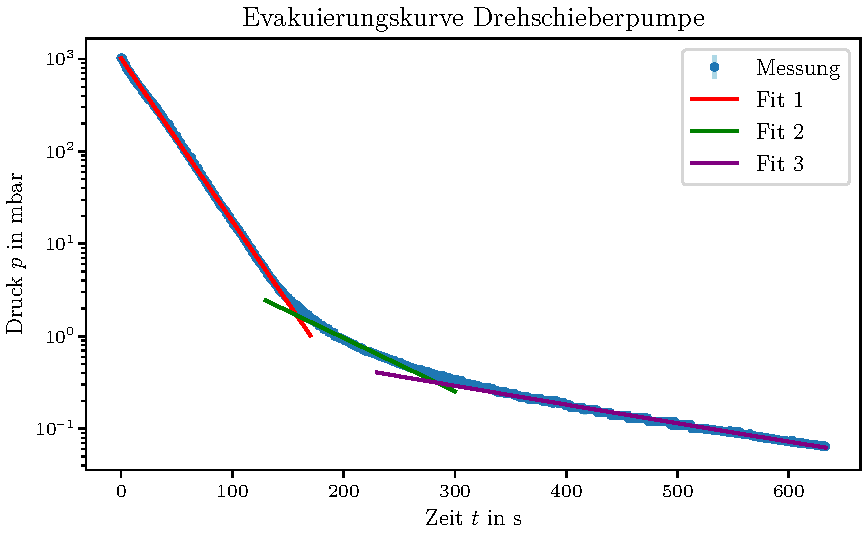
\includegraphics[width=\textwidth]{plots/DP_Evakuierungskurve.pdf}
    \caption{Evakuierungskurve der Drehschieberpumpe mit drei Fitkurven.}
    \label{fig:DP_evak}
\end{figure}

Die berechneten Fitparameter bestimmen sich zu 
\begin{align}
    m_1 = \qty[separate-uncertainty=false]{-0.0408(7)}{\milli\bar\per\second}, & b_1 = \qty[separate-uncertainty=false]{0.01(7)}{\milli\bar} \\
    m_2 = \qty[separate-uncertainty=false]{-0.01441(34)}{\milli\bar\per\second}, & b_2 = \qty[separate-uncertainty=false]{-4.16(8)}{\milli\bar}\\
    m_3 = \qty[separate-uncertainty=false]{-0.005970(4)}{\milli\bar\per\second}, & b_3 = \qty[separate-uncertainty=false]{-6.174(6)}{\milli\bar}.
\end{align}

Für die erste Gerade werden die ersten 150 Datenpunkte ausgewertet, für die zweite die nächsten 100 und für die dritte alle nachfolgenden Punkte.

Nach \eqref{eq:S_evak} ergibt sich
\begin{align}
    S_1 &= (\num{1.39} \pm \num{0.14}) \si{\liter\per\second} \\
    S_2 &= (\num{0.49} \pm \num{0.05}) \si{\liter\per\second} \\
    S_3 &= (\num{0.41} \pm \num{0.04}) \si{\liter\per\second} 
\end{align}
%%% HIER NOCH DIE GENAUEN GÜLTIGKEITSBEREICHE AUSRECHNEN? t = b1 - b2 / (m2 - m1)
$S_1$ hat dabei einen Gültigkeitsbereich von $\SI{1000}{\milli\bar}$ bis $\SI{2}{\milli\bar}$, $S_2$ von $\SI{2}{\milli\bar}$ bis $\SI{0.3}{\milli\bar}$ und $S_3$ darunter.

\subsubsection{Leckratenmessungen für bestimmte Gleichgewichtsdrücke $p_\text{G}$}

Für $p_\text{G} = \SI{100}{\milli\bar}$ werden drei Messungen durchgeführt und ein Mittelwert ausgewertet. Die anderen Gleichgewichtsdrücke werden nur einmal gemessen, da die statistische Abweichung, wie gezeigt wird, ausreichend gering ist.

Die Messungen für $\SI{100}{\milli\bar}$ finden sich in Abbildung \ref{fig:DP_leck_100mbar_alle}

\begin{figure}[H]
    \centering
    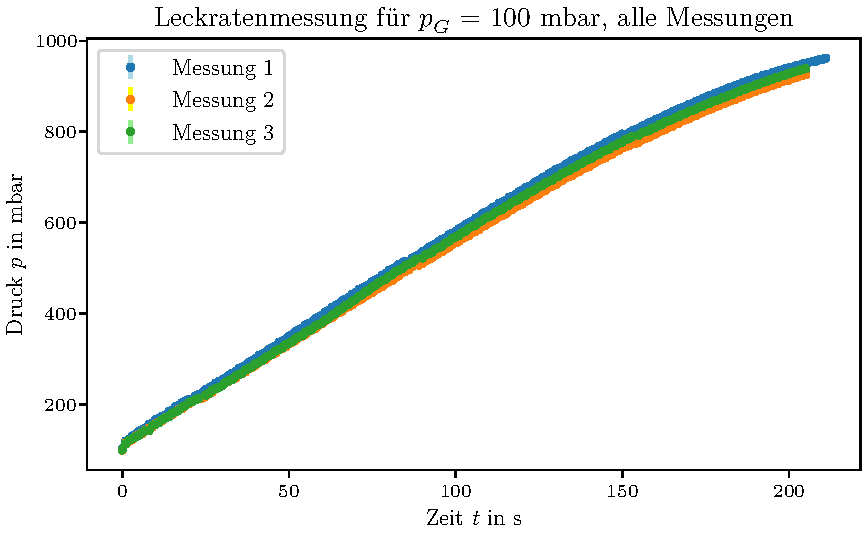
\includegraphics[width=\textwidth]{plots/DP_Leck_100mbar_alle.pdf}
    \caption{Drei Leckratenmessungen bei $p_\text{G} = \qty{100}{\milli\bar}$.}
    \label{fig:DP_leck_100mbar_alle}
\end{figure}

Für den Mittelwert ergibt sich die Grafik in Abbildung \ref{fig:DP_Leck_100mbar_mittelwert}.

\begin{figure}[H]
    \centering
    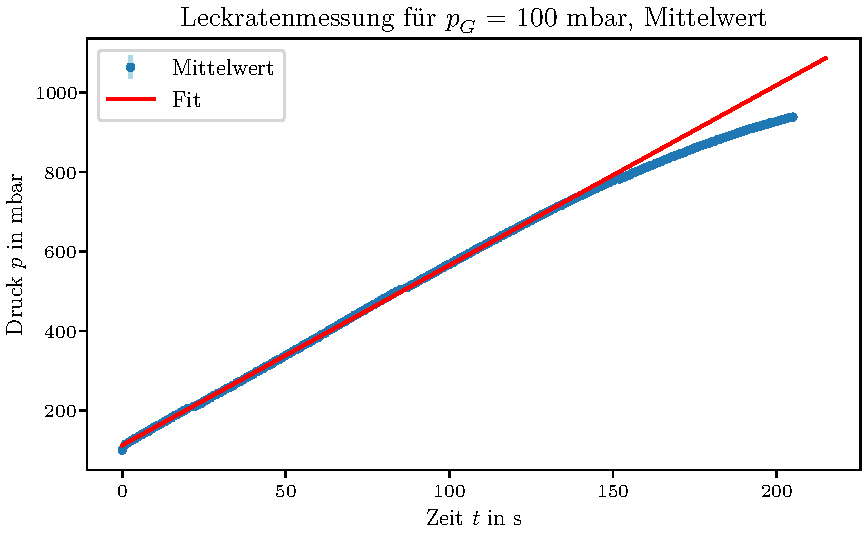
\includegraphics[width=\textwidth]{plots/DP_Leck1_100mbar_mittelwert.pdf}
    \caption{Mittelwerte der drei Messreihen.}
    \label{fig:DP_Leck_100mbar_mittelwert}
\end{figure}

Die Parameter des Fits lauten 
\begin{equation}
    m = \qty{4.5283(3)}{\milli\bar\per\second}, \. b = \qty{112.640(18)}{\milli\bar},
\end{equation}
wobei nur die Messwerte zwischen dem 10. und 150. Messwert
für die Regression benutzt werden.

Es ergibt sich ein Saugvermögen von
\begin{equation}
    S_{100} = (\num{1.54} \pm \num{0.16}) \si{\liter\per\second}.
\end{equation}

Für $p_\text{G} = \SI{50}{\milli\bar}$ ergibt sich die Grafik in Abbildung \ref{fig:DP_Leck_50mbar_mittelwert}.

\begin{figure}[H]
    \centering
    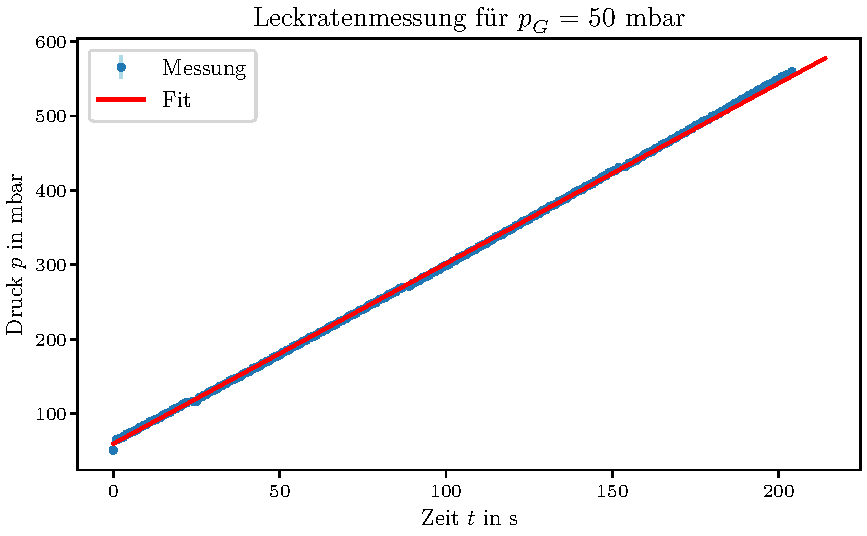
\includegraphics[width=\textwidth]{plots/DP_Leck_50mbar.pdf}
    \caption{Mittelwerte der drei Messreihen.}
    \label{fig:DP_Leck_50mbar_mittelwert}
\end{figure}

Die Parameter des Fits lauten 
\begin{equation}
    m = \qty{2.419(1)}{\milli\bar\per\second}, \. b = \qty{59.78(7)}{\milli\bar},
\end{equation}
wobei nur die Werte nach der 10. Messung
für die Regression benutzt werden.

Es ergibt sich ein Saugvermögen von
\begin{equation}
    S_{50} = (\num{1.64} \pm \num{0.17}) \si{\liter\per\second}.
\end{equation}

Für $p_\text{G} = \SI{10}{\milli\bar}$ ergibt sich die Grafik in \ref{fig:DP_Leck_10mbar_mittelwert}.

\begin{figure}[H]
    \centering
    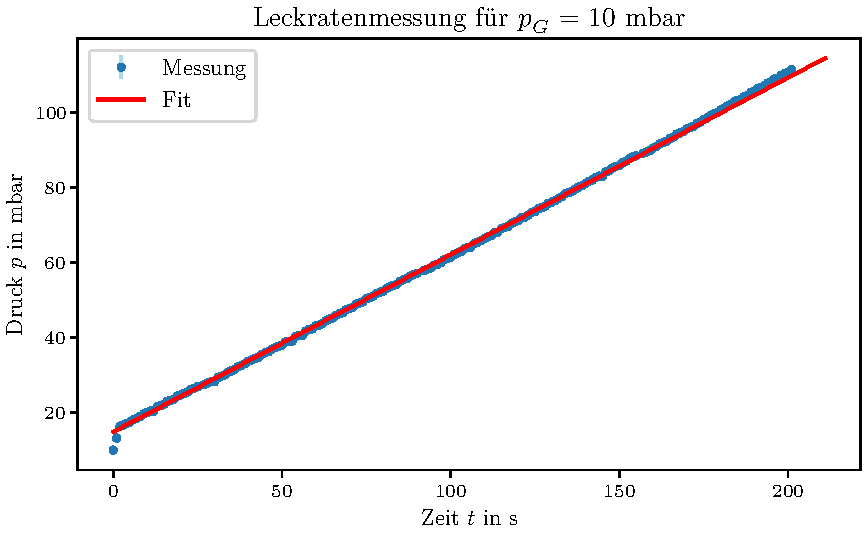
\includegraphics[width=\textwidth]{plots/DP_Leck_10mbar.pdf}
    \caption{Mittelwerte der drei Messreihen. Fit: $m = \num{0.47184} \pm \num{0.00022}$, $b = \num{14.886} \pm \num{0.016}$.}
    \label{fig:DP_Leck_10mbar_mittelwert}
\end{figure}

Die Parameter des Fits lauten 
\begin{equation}
    m = \qty{0.47184(22)}{\milli\bar\per\second}, \. b = \qty{14.886(16)}{\milli\bar},
\end{equation}
wobei nur die Werte nach der 10. Messung
für die Regression benutzt werden.

Es ergibt sich ein Saugvermögen von
\begin{equation}
    S_{10} = (\num{1.60} \pm \num{0.17}) \si{\liter\per\second}.
\end{equation}

Für $p_\text{G} = \SI{0.5}{\milli\bar}$ ergibt sich die Grafik in Abbildung \ref{fig:DP_Leck_05mbar_mittelwert}.

\begin{figure}[H]
    \centering
    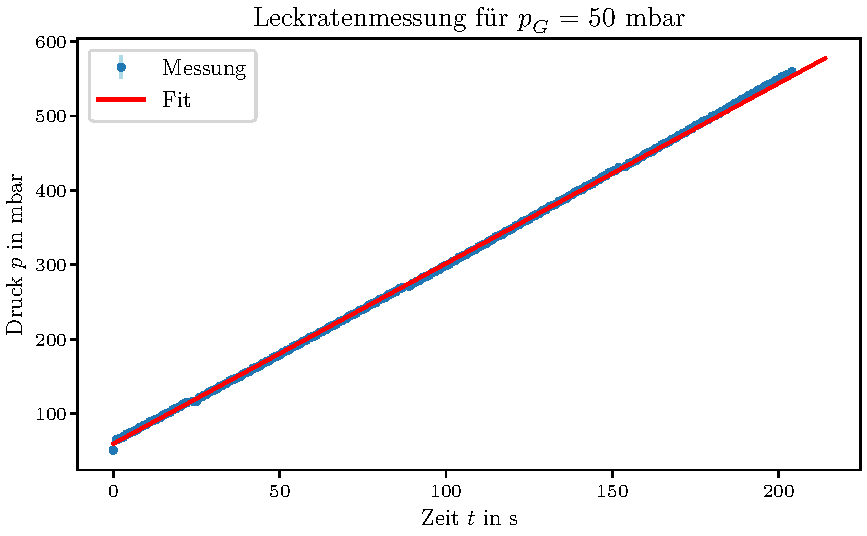
\includegraphics[width=\textwidth]{plots/DP_Leck_50mbar.pdf}
    \caption{Mittelwerte der drei Messreihen.}
    \label{fig:DP_Leck_05mbar_mittelwert}
\end{figure}

Die Parameter des Fits lauten 
\begin{equation}
    m = \qty{0.0150(4)}{\milli\bar\per\second}, \. b = \qty{1.63(4)}{\milli\bar},
\end{equation}
wobei nur die Werte nach der 10. Messung
für die Regression benutzt werden.

Es ergibt sich ein Saugvermögen von
\begin{equation}
    S_{\num{0.5}} = (\num{1.02} \pm \num{0.15}) \si{\liter\per\second}.
\end{equation}



\subsection{Turbomolekularpumpe}

Der für die Turbomolekularpumpe gemessene Enddruck beträgt
\begin{equation}
    p_\text{E} = (\num{5.0} \pm \num{1.5}) \cdot 10^{-5} \, \si{\milli\bar}.\\
\end{equation}
Das Volumen wird der Versuchsanleitung entnommen und beträgt
\begin{equation}
    V_\text{TP} = (\num{33} \pm \num{3.3}) \, \si{\liter}.
\end{equation}

\subsubsection{Evakuierungskurve}
Für die Evakuierungskurve werden drei Messreihen aufgenommen, bei der der Rezipient von einem Startdruck von ungefähr $p_0 = \num{5} \cdot 10^{-3} \, \si{\milli\bar}$ evakuiert wird.
Diese sehen wie in Abbildung \ref{fig:TP_evak_alle} aufgezeigt aus.

\begin{figure}[H]
    \centering
    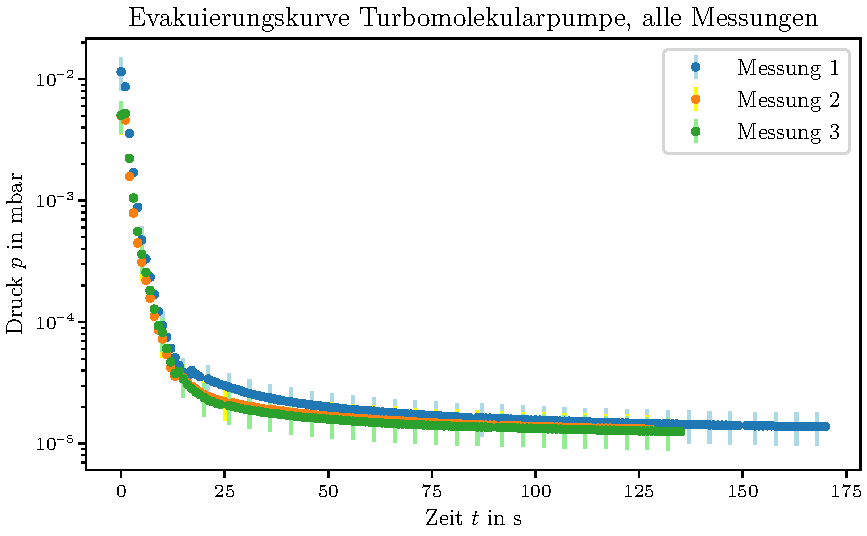
\includegraphics[width=\textwidth]{plots/TP_Evakuierungskurve_alle.pdf}
    \caption{Drei Evakuierungskurven der Turbomolekularpumpe.}
    \label{fig:TP_evak_alle}
\end{figure}

Alle Kurven haben einen kleinen Sprung, die blaue Kurve bei $t = \SI{20}{\second}$, die grüne und orangene bei $t = \SI{15}{\second}$.
Für die Mittelwertbildung wird die blaue Kurve ignoriert. \\
Es ergibt sich die Grafik in Abbildung \ref{fig:TP_evak}.

\begin{figure}[H]
    \centering
    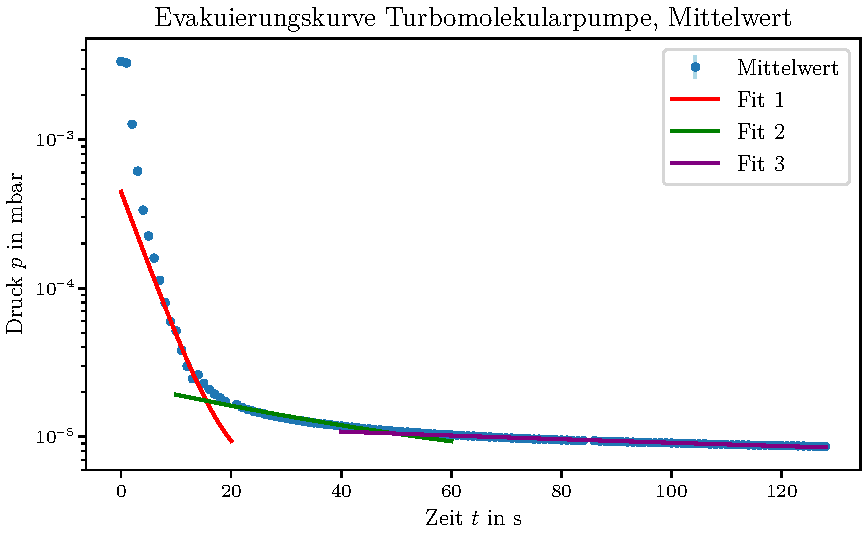
\includegraphics[width=\textwidth]{plots/TP_Evakuierungskurve.pdf}
    \caption{Evakuierungskurve der Turbomolekularpumpe mit drei Fitkurven.}
    \label{fig:TP_evak}
\end{figure}

Die berechneten Fitparameter bestimmen sich zu 
\begin{align}
    m_1 = \qty[separate-uncertainty=false]{-0.2304202(4)}{\milli\bar\per\second}, & b_1 = \qty[separate-uncertainty=false]{2.030883(5)}{\milli\bar} \\
    m_2 = \qty[separate-uncertainty=false]{-0.023777465(13)}{\milli\bar\per\second}, & b_2 = \qty[separate-uncertainty=false]{-5.2276858(5)}{\milli\bar}\\
    m_3 = \qty[separate-uncertainty=false]{-0.0058313180(27)}{\milli\bar\per\second}, & b_3 = \qty[separate-uncertainty=false]{-6.12055098(26)}{\milli\bar}.
\end{align}

Für die erste Gerade werden die ersten 15 Messpunkte verwendet, für die zweite Gerade die nächsten 35 und für die dritte Gerade die restlichen Punkte.

Nach \eqref{eq:S_evak} ergibt sich
\begin{align}
    S_1 &= (\num{7.5} \pm \num{0.8}) \si{\liter\per\second} \\
    S_2 &= (\num{0.78} \pm \num{0.08}) \si{\liter\per\second} \\
    S_3 &= (\num{0.192} \pm \num{0.019}) \si{\liter\per\second} 
\end{align}

$S_1$ hat dabei einen Gültigkeitsbereich bis $\num{2}\cdot 10^{-4} \, \si{\milli\bar}$, $S_2$ von $\num{2}\cdot 10^{-5} \, \si{\milli\bar}$ bis $10^{-5} \si{\milli\bar}$ und $S_3$ darunter.

\subsubsection{Leckratenmessungen für bestimmte Gleichgewichtsdrücke $p_\text{G}$}

Für $p_\text{G} = 10^{-4} \, \si{\milli\bar}$ ergibt sich die Grafik in Abbildung \ref{fig:TP_Leck_1e4}.

\begin{figure}[H]
    \centering
    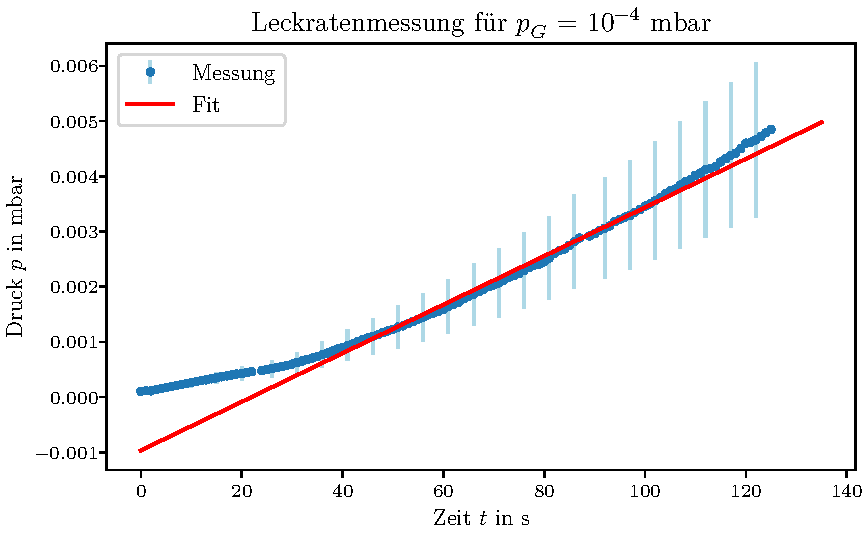
\includegraphics[width=\textwidth]{plots/TP_Leck_1e4.pdf}
    \caption{Leckratenmessung mit Fit.}
    \label{fig:TP_Leck_1e4}
\end{figure}

Die Parameter des Fits lauten 
\begin{equation}
    m = \qty{4.40(32)}{\milli\bar\per\second}, b = \qty{-9.7(21)e-4}{\milli\bar},
\end{equation}
wobei nur die Werte nach dem 40. Messpunkt
für die Regression benutzt werden.

Es ergibt sich ein Saugvermögen von
\begin{equation}
    S_{10^{-4}} = (\num{15} \pm \num{5}) \si{\liter\per\second}.
\end{equation}

Für $p_\text{G} = 2 \cdot 10^{-4} \, \si{\milli\bar}$ ergibt sich die Grafik in Abbildung \ref{fig:TP_Leck_2e4}.

\begin{figure}[H]
    \centering
    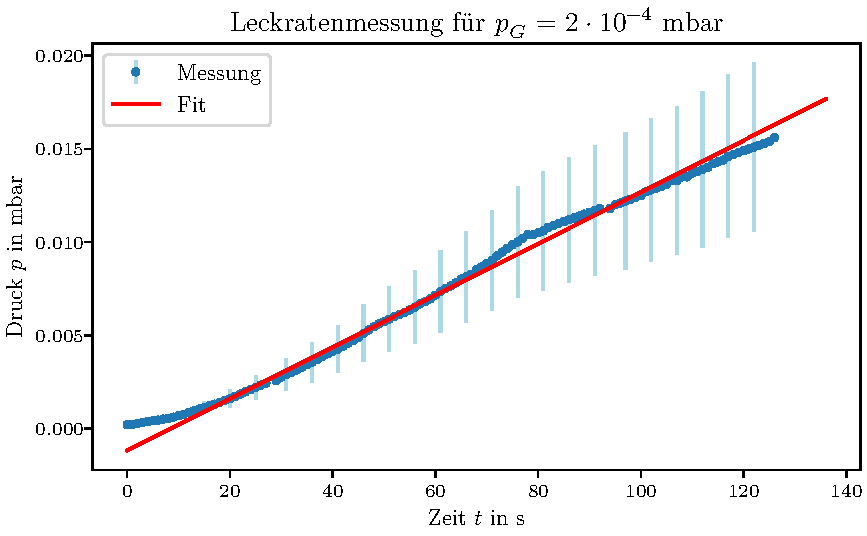
\includegraphics[width=\textwidth]{plots/TP_Leck_2e4.pdf}
    \caption{Leckratenmessung mit Fit.}
    \label{fig:TP_Leck_2e4}
\end{figure}

Die Parameter des Fits lauten 
\begin{equation}
    m = \qty{13.9(12)e-5}{\milli\bar\per\second}, b = \qty{1.2(8)e-4}{\milli\bar},
\end{equation}
wobei nur die Werte nach dem 40. Messpunkt
für die Regression benutzt werden.

Es ergibt sich ein Saugvermögen von
\begin{equation}
    S_{2 \cdot 10^{-4}} = (\num{23} \pm \num{8}) \si{\liter\per\second}.
\end{equation}

Für $p_\text{G} = 5 \cdot 10^{-5} \, \si{\milli\bar}$ ergibt sich die Grafik in Abbildung \ref{fig:TP_Leck_5e5}.

\begin{figure}[H]
    \centering
    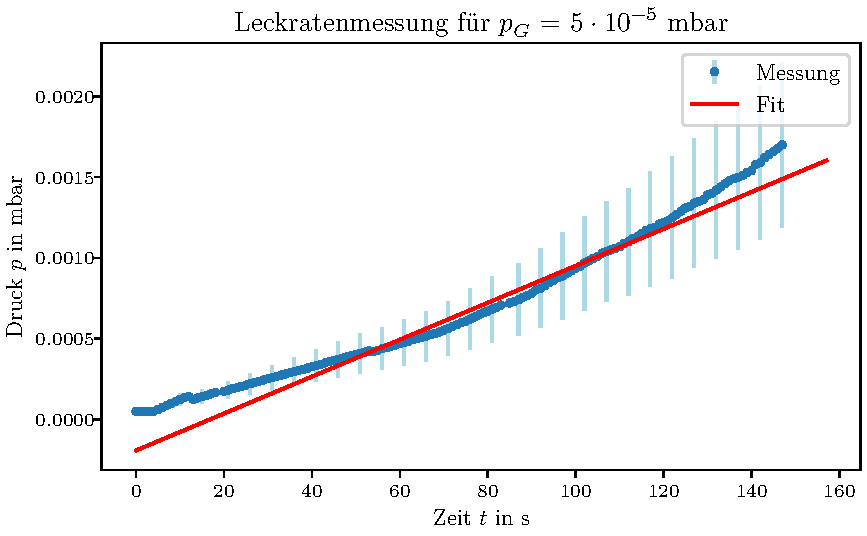
\includegraphics[width=\textwidth]{plots/TP_Leck_5e5.pdf}
    \caption{Leckratenmessung mit Fit.}
    \label{fig:TP_Leck_5e5}
\end{figure}

Die Parameter des Fits lauten 
\begin{equation}
    m = \qty{1.14(8)e-5}{\milli\bar\per\second}, b = \qty{-1.9(6)e-4}{\milli\bar},
\end{equation}
wobei nur die Werte nach dem 40. Messpunkt
für die Regression benutzt werden.

Es ergibt sich ein Saugvermögen von
\begin{equation}
    S_{5 \cdot 10^{-5}} = (\num{7.5} \pm \num{2.4}) \si{\liter\per\second}.
\end{equation}

Für $p_\text{G} = 7 \cdot 10^{-5} \, \si{\milli\bar}$ ergibt sich die Grafik in Abbildung \ref{fig:TP_Leck_7e5}.

\begin{figure}[H]
    \centering
    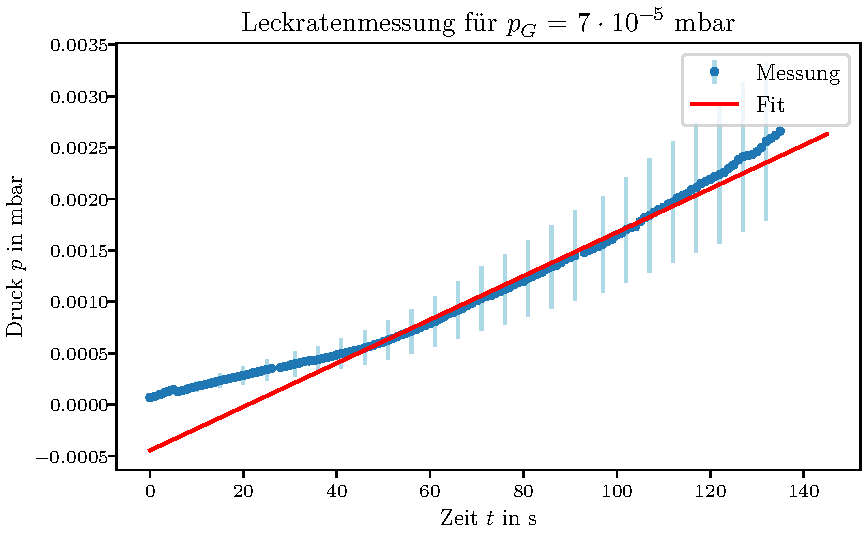
\includegraphics[width=\textwidth]{plots/TP_Leck_7e5.pdf}
    \caption{Leckratenmessung mit Fit.}
    \label{fig:TP_Leck_7e5}
\end{figure}

Die Parameter des Fits lauten 
\begin{equation}
    m = \qty{2.12(14)e-5}{\milli\bar\per\second}, b = \qty{-4.5(10)e-4}{\milli\bar},
\end{equation}
wobei nur die Werte nach dem 40. Messpunkt
für die Regression benutzt werden.

Es ergibt sich ein Saugvermögen von
\begin{equation}
    S_{7 \cdot 10^{-5}} = (\num{10} \pm \num{3.2}) \si{\liter\per\second}.
\end{equation}



\subsection{Leitwertbestimmung eines kurzen Rohres}

Es werden zwei Leckratenmessungen für den Aufbau mit einem kurzen Verbindungsrohr bei zwei verschiedenen Drücken durchgeführt.
Die zwei Messgeräte D1 und D2 werden ausgelesen und ihre Messwerte miteinander verglichen.

Für $p_\text{G} = 2 \cdot 10^{-4} \, \si{\milli\bar}$ ergibt sich die Grafik in Abbildung \ref{fig:Leitparam_2e4}.

\begin{figure}[H]
    \centering
    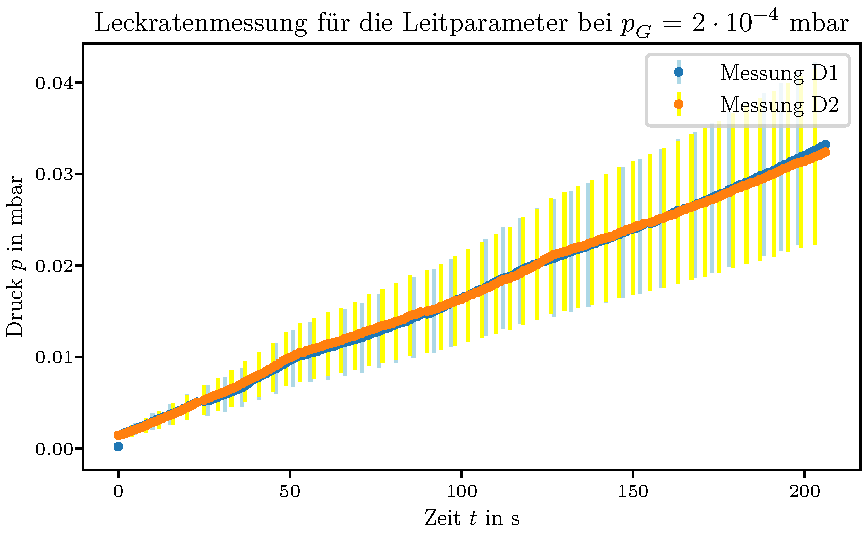
\includegraphics[width=\textwidth]{plots/Leitparam_2e4.pdf}
    \caption{Leckratenmessung für den Leitparameter. Die Leckraten sind nahezu identisch.}
    \label{fig:Leitparam_2e4}
\end{figure}

Die Parameter des Fits lauten 
\begin{equation}
    m = \qty{1.61(6)}{\milli\bar\per\second}, \. b = \qty{1.1(4)e-4}{\milli\bar},
\end{equation}
wobei nur die Werte nach dem 20. Messpunkt
für die Regression benutzt werden.

Für $p_\text{G} = 5 \cdot 10^{-5} \, \si{\milli\bar}$ ergibt sich folgende Grafik.

\begin{figure}[H]
    \centering
    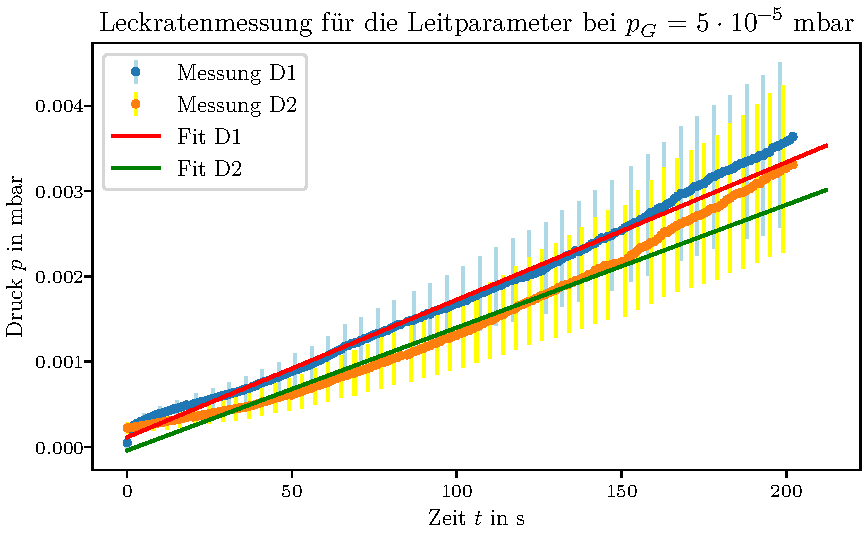
\includegraphics[width=\textwidth]{plots/Leitparam_5e5.pdf}
    \caption{Lekratenmessung für den Leitparameter. Die Leckraten sind unterschiedlich.}
    \label{fig:Leitparam_5e5}
\end{figure}

Die Parameter des Fits lauten 
\begin{align}
    m_1 = \qty{1.61(6)e-5}{\milli\bar\per\second}, & \. b_1 = \qty{1.1(4)e-4}{\milli\bar} \\
    m_2 = \qty{1.44(6)e-5}{\milli\bar\per\second}, & \. b_2 = \qty{-4(4)e-5}{\milli\bar}.
\end{align}
wobei nur die Werte nach dem 20. Messpunkt
für die Regression benutzt werden.

Es ergeben sich Saugvermögen von
\begin{align}
    S_{\text{Leitwert, D1}} &= (\num{2.7} \pm \num{0.8}) \si{\liter\per\second} \\
    S_{\text{Leitwert, D2}} &= (\num{2.4} \pm \num{0.8}) \si{\liter\per\second}.
\end{align}

Wird $S_{\text{Leitwert, D2}}$ als das effektive Saugvermögen $S_\text{eff}$ und $S_{\text{Leitwert, D1}}$ als das theoretische Saugvermögen angenommen, ist 
\begin{equation}
    \frac{1}{S_\text{eff}} = \frac{1}{S} + \frac{1}{L}
\end{equation}
eine Abschätzung für den Leitwert $L$, hier
\begin{equation}
    L = (20 \pm 80) \, \si{\liter\per\second}
\end{equation}

